\section{Camera Module}

Camera modules have become integral components in various embedded systems, enabling devices to capture images and video for processing and analysis. These modules are typically made up of an image sensor, lens, and support circuitry, which allow them to interface with microcontrollers, single-board computers, and other embedded platforms. Camera modules are often classified based on their resolution, power consumption, compatibility with specific devices, and imaging quality. The OV series of camera modules from OmniVision, a prominent supplier of CMOS image sensors, are particularly popular in applications ranging from surveillance to IoT and computer vision. Below, we discuss three widely used models: the OV2640, OV7670, and OV5640.

\subsection{OV2640}
The OV2640 is a compact, low-power camera module with a 2-megapixel (1600 x 1200 pixels) CMOS sensor. This module is widely used in embedded applications due to its energy efficiency and compatibility with microcontrollers, particularly the ESP32. The OV2640 supports image output formats like JPEG, YUV, and RGB, making it versatile for different applications. It operates effectively at lower resolutions, allowing faster processing and reduced memory usage, which is essential in IoT devices that require minimal power. Additionally, the OV2640 includes support for automatic white balance, exposure control, and other image enhancements, allowing it to capture acceptable quality images in various lighting conditions.\cite{OV2640}
\begin{figure}[h]
	\centering
	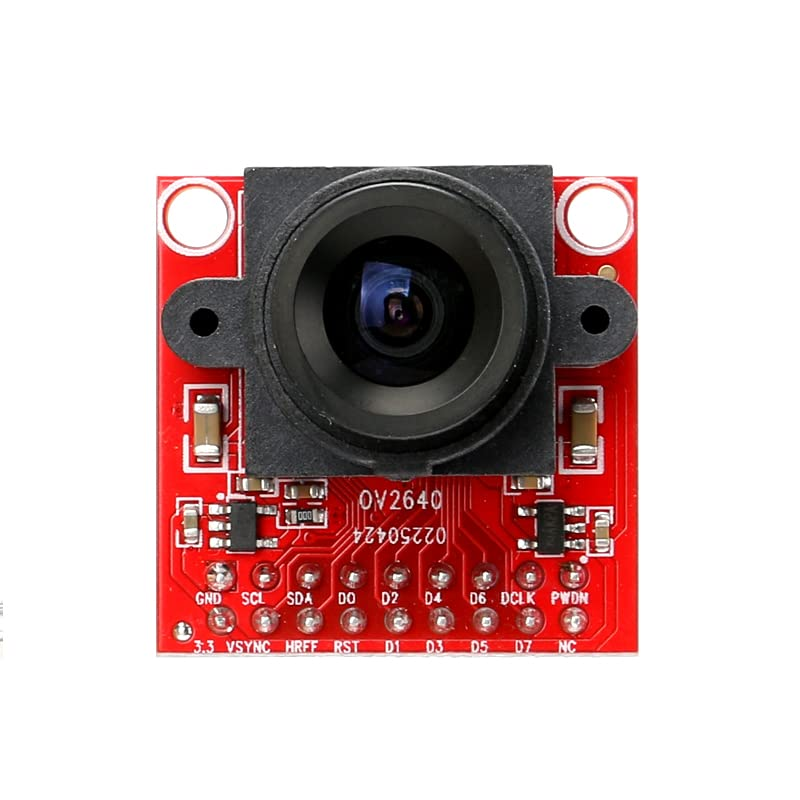
\includegraphics[width=0.5\linewidth]{assets/ch2/OV2640}
	\caption{OV2460 Camera Module}
	\label{fig:ov2640}
\end{figure}


\subsection{OV7670}
The OV7670 is a low-cost VGA (640 x 480 pixels) camera module often chosen for applications requiring basic image capture, particularly where high resolution is not a priority. With its 0.3-megapixel sensor, the OV7670 is suitable for simpler image processing tasks, such as color tracking, object detection, and line following, often found in educational and hobbyist projects. The OV7670 is compatible with many microcontrollers, like the Arduino, due to its relatively low data and power requirements. Although it lacks some of the advanced features found in newer modules, it still offers functionalities such as image scaling, automatic white balance, and gamma correction, making it a viable choice for cost-sensitive and low-power applications. \cite{OV7670}
\begin{figure}[h]
	\centering
	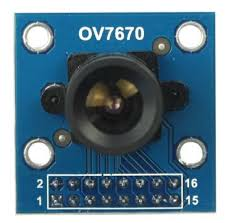
\includegraphics[width=0.5\linewidth]{assets/ch2/OV7670}
	\caption{OV7670 Camera Module}
	\label{fig:ov7670}
\end{figure}


\subsection{OV5640}
The OV5640 is a high-resolution camera module with a 5-megapixel (2592 x 1944 pixels) CMOS sensor. It is favored for applications requiring detailed images, such as facial recognition, barcode scanning, and other computer vision tasks. This module provides a range of image formats, including JPEG, RAW, and YUV, and supports video output at different frame rates, depending on the resolution. The OV5640 also features advanced imaging controls like autofocus, which can enhance the clarity and quality of images in diverse environments. Due to its higher resolution and additional features, the OV5640 requires more processing power and memory, making it suitable for platforms like Raspberry Pi and other single-board computers capable of handling high-definition image processing. \cite{OV5640}

\begin{figure}[h]
	\centering
	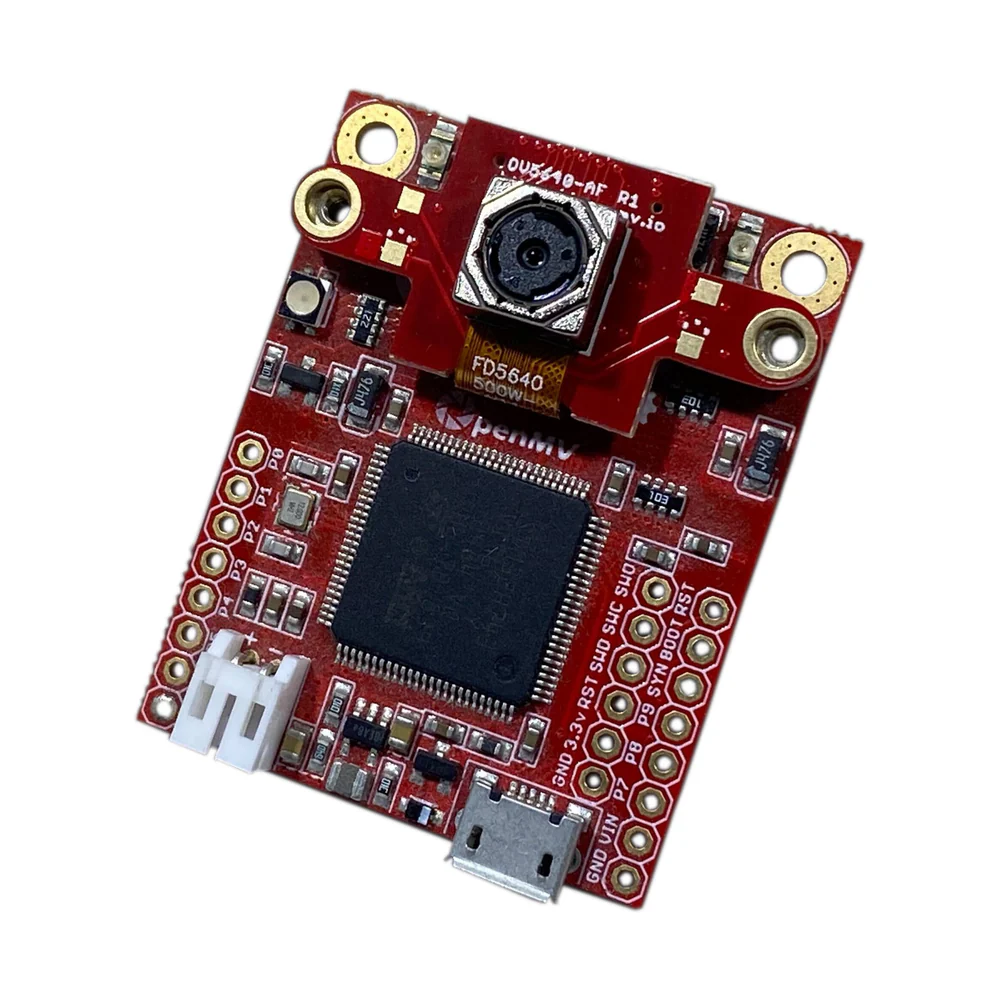
\includegraphics[width=0.5\linewidth]{assets/ch2/OV5640}
	\caption{OV5640 Camera Module}
	\label{fig:ov5640}
\end{figure}



